
Originally the package was structured around two classes, \textit{FDataGrid} and
\textit{FDataBasis}, designed for each of the main data representations of the data and
consisted of four modules with basic statistics, operations and methods to
perform kernel smoothing.

\begin{figure}[Map of scikit-fda]{FIG:SCIKITMAP}{Map of scikit-fda \cite{ramos-carrenoScikitfdaPythonPackage2019}}
	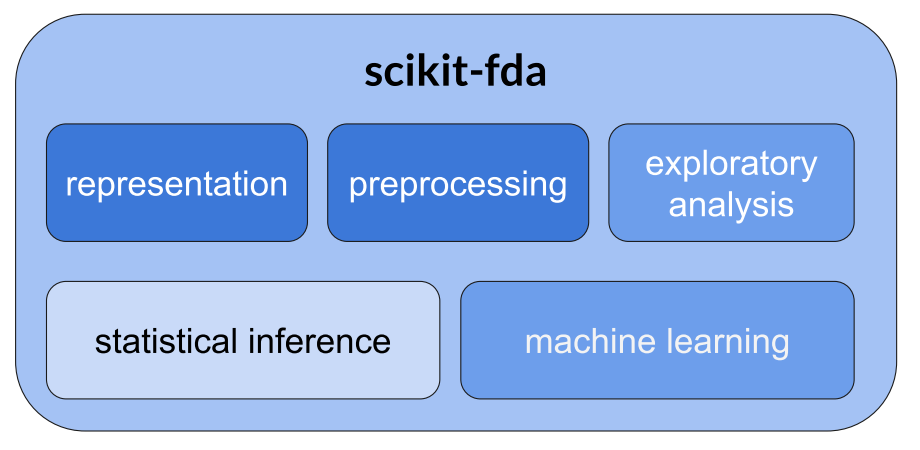
\includegraphics[width=10cm]{scikit-map}
\end{figure}


Due to the expansion of the project, the package has been completely
restructured, with a more hierarchical structure. Figure \ref{FIG:SCIKITMAP}
shows a diagram with a high-level description of this structure. Darker colors in the figure represent a more advanced stage of development of the modules.
The following
subsections summarize, in general terms, the functionalities incorporated and
design changes made during this work. A more detailed description of the functions and classes developed may be found
in Annex \ref{CAP:GUIDE}, or in the online documentation, available at \href{https://fda.readthedocs.io/}{fda.readthedocs.io}.
